\section{Experimentación}
Llegado el momento de la experimentación, se tenía una base de datos de imágenes divididas entre
resoluciones de 112 x 92 píxeles y de 28 x 23 píxeles y se decidió divivir los tests de igual forma.

A los tests hechos sobre las imágenes de 28 x 23 se los subdividió en dos, tests con el método 0 y
tests con el método 1. Esto hace referencia al método empleado para buscar los autovectores y
autovalores de la matriz de covarianzas. El método 0 consistía en hacerlo sobre la matriz $A^t A$
mientras que el método 1 consistía en hacerlo sobre la matriz $A A^t$.

Por el lado de las imágenes de 112 x 92 pixeles se volvió inviable el método 0, dado que la
dimension de la matriz terminaría siendo de $(112*92)^2 > 106$ millones de celdas mientras que la
matriz del método 1 tendría \textbf{cómo máximo} $(41*10)^2 = 168 100$ celdas si usamos a todas las
imágenes.

En cada una de las subdivisiones se testeó lo siguiente al ir aumentando el K, o la cantidad de
autovectores:
\begin{compactitem}
  \item \textbf{Mediciones de TK}: mide el tiempo de obtener la matriz de autovectores. Es decir:
  \begin{compactenum}
    \item Restarle el $\mu$ y dividir por $\sqrt{n-1}$ a la matriz
    \item Tiempo de calcular los K autovectores
    \item Tiempo de multiplicar por izquierda al autovector de $A A^t$ por $A^t$ para obtener el
    autovector con el mismo autovalor pero de $A^t A$.
  \end{compactenum}
  Se varía entre 1, 5 y 10 muestras para 11, 21 y 41 personas.
  \item \textbf{Mediciones de Ttodos}: el tiempo de identificar a todos los sujetos usando el método
  de identificación del vecino más cercano. Incluye el tiempo de restarle el $\mu$ y dividir por
  $\sqrt{n-1}$ a la matriz. Se varía entre 1, 5 y 10 muestras para 11, 21 y 41 personas.
  \item \textbf{Mediciones de Tcentro}: el tiempo de identificar a todos los sujetos usando el método
  de identificación de los centros de masa. Incluye el tiempo de restarle el $\mu$ y dividir por
  $\sqrt{n-1}$ a la matriz. Se varía entre 1, 5 y 10 muestras para 11, 21 y 41 personas.
  \item \textbf{Mediciones de HitsTodos}: el coeficiente entre los \textit{hits} al identificar un
  sujeto y la cantidad de estos usando el método del vecino más cercano. Se varía entre 1, 3, 5, 7,
  9 y 10 muestras para 11, 21 y 41 personas.
  \item \textbf{Mediciones de HitsCentro} el coeficiente entre los \textit{hits} al identificar un
  sujeto y la cantidad de estos usando el método de los centros de masa. Se varía entre 1, 3, 5, 7,
  9 y 10 muestras para 11, 21 y 41 personas.
\end{compactitem}

Para los tests, eligiremos mostrar cómo se irán comportando estas mediciones acorde aumente el K.
Además, para una cantidad fija de personas, cuando decimos, por ejemplo, \textit{se varía
  entre 1, 5 y 10 muestras}, nos referimos a que medimos 3 instancias distintas. La primera, con una
muestra, se refiera a que de la base de datos se elige aleatoriamente una muestra por cada persona
para calcular la matriz inicial y, por ende, la matriz de autovectores. Además, se elige para
identificar por cada persona una muestra que no haya sido usada para generar la matriz inicial. En
el caso de 5 muestras, se genera la matriz usando 5 muestras por persona y de nuevo por cada una de
las personas tenidas en cuenta, se trata de identificar una de sus muestras que no haya sido usada
para calcular la matriz inicial.

El caso \textbf{distinto} sería el caso de 10 muestras. Aquí, dado que se usan todas las muestras
disponibles para cada una de las personas para generar la matriz inicial, no quedan muestras libres
para identificar por cada persona. En ese caso se elige una muestra random y se testea qué tan
buenos son los métodos de reconocimiento cuando se trata de identificar a alguien perteneciente a la
base de datos.


% Con muestras nos referimos a cantidad de muestras por persona usadas para calcular la matriz de
% autovectores. En el caso de las personas a identificar, se elige una muestra random que no haya sido
% usada en el cálculo de los autovectores.

Sobre estos tests esperamos encontrar que:
\begin{compactitem}
  \item Los tiempos son crecientes acorde al incremento de los autovectores buscados dado que
  mientras más grande sea la matriz de autovectores, más tiempo se tardará en encontrarla y, en el
  caso del método 1, se deberá multiplicar por izquierda a cada autovector para trasladarlo a un
  autovector de la matriz de $A^t A$.
  \item Los tiempos del método 1 deben ser mucho menores a los tiempos del método 0.
  \item El coeficiente de HitsTodos debe ser siempre 1 para los casos en los que se usen 10 muestras
  dado que toda muestra a identificar ha sido usada para generar la matriz de autovectores y,
  además, este método de identificación compara con todos los puntos, y entre ellos va a estar él
  mismo, que terminaría siendo el más cercano.
  \item Los coeficientes de HitsTodos y HitsCentro deben aumentar acorde aumenten la cantidad de
  muestras y la cantidad de autovectores.
\end{compactitem}


\section{Resultados}
\subsection{Experimentaci\'on con Imagenes Reducidas}
\subsubsection{M\'etodo 0: Utilizando $A^tA$}

\textbf{Mediciones de TK}
\begin{figure}[H]
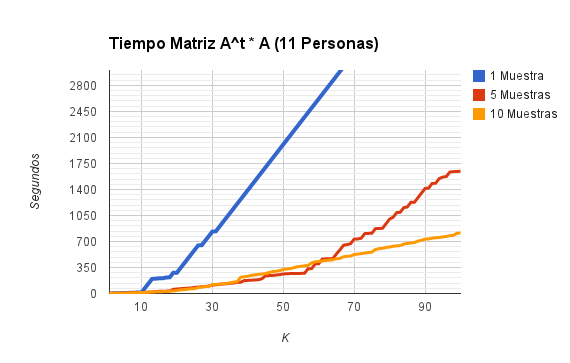
\includegraphics[width=0.95\textwidth]{img/image1.png}
     \caption{Tiempos Matrix $A^tA$ con 11 personas variando K}
\end{figure}

\begin{figure}[H]
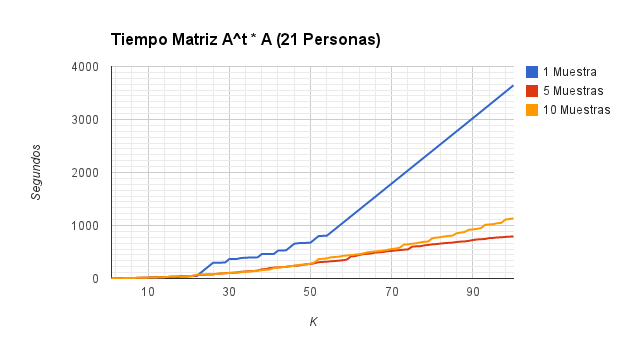
\includegraphics[width=0.95\textwidth]{img/image2.png}
     \caption{Tiempos Matrix $A^tA$ con 21 personas variando K}
\end{figure}

\begin{figure}[H]
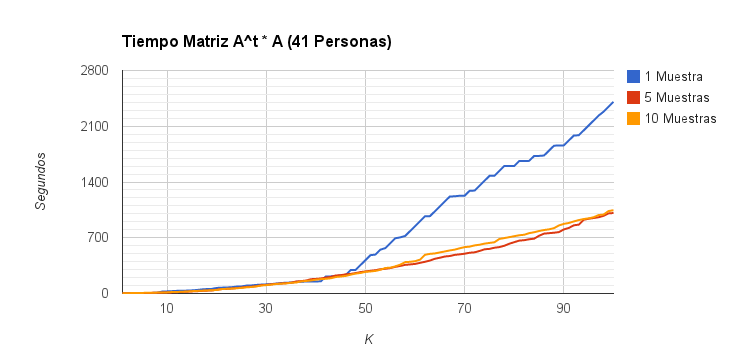
\includegraphics[width=0.95\textwidth]{img/image3.png}
     \caption{Tiempos Matrix $A^tA$ con 41 personas variando K}
\end{figure}

Algo que en un principio parecería muy extraño es que el tiempo de calcular la matriz crece
inversamente proporcional a la cantidad de muestras, sin ningún sentido obvio. Pero, si nos ponemos
a analizar los tests, sabemos que el tamaño de la matriz es igual para todos los casos ya que $A^tA$
siempre es de $DimImg \times DimImg$, lo que var\'ia es que la cantidad de autovalores no nulos es a
lo sumo la cantidad de imagenes en la base de datos, o sea, esta acotado por $Muestras \times
Personas$. Esto \'ultimo se traduce en que al pretender calcular m\'as autovalores, el m\'etodo de
la potencia no converja. Es as\'i que como se ve en la gr\'afico de 11 personas, se ve esta
divergencia en k = 11 y k = 55,\footnote{Calculado como $Muestras \times Personas$, cota de
  autovalores} para 1 Muestra y 5 Muestras respectivamente.

Además, vemos que el tiempo crece con los K, totalmente intuitivo.

\textbf{Mediciones de Ttodos }

\begin{figure}[H]
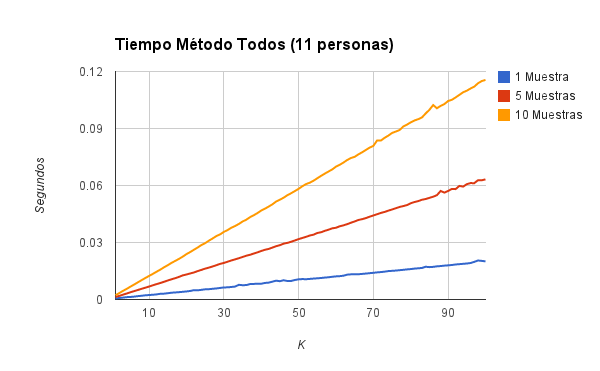
\includegraphics[width=1\textwidth]{img/image4.png}
     \caption{Tiempos Todos con Matrix $A^tA$ con 11 personas variando K}
\end{figure}

\begin{figure}[H]
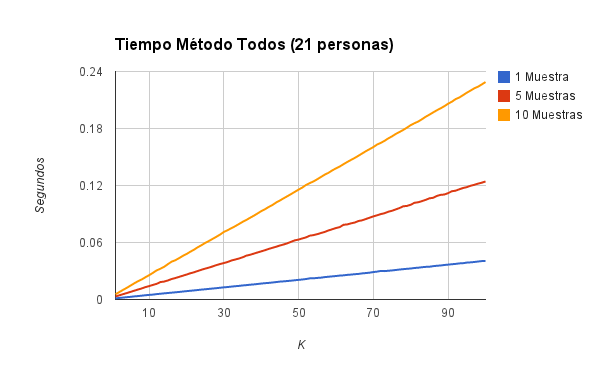
\includegraphics[width=1\textwidth]{img/image5.png}
     \caption{Tiempos Todos con Matrix $A^tA$ con 21 personas variando K}
\end{figure}

\begin{figure}[H]
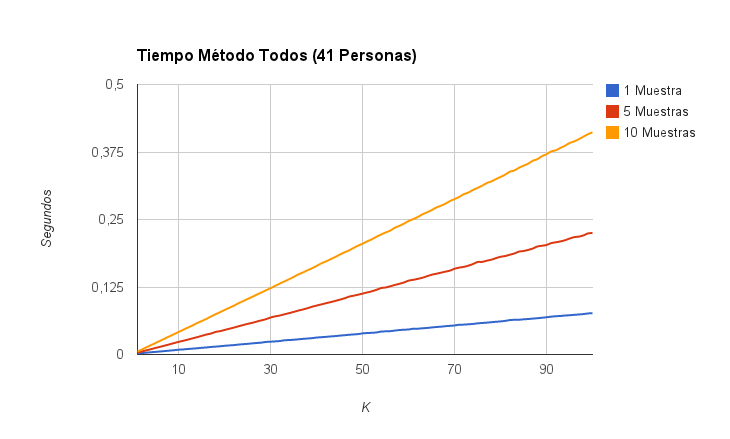
\includegraphics[width=1\textwidth]{img/image6.png}
     \caption{Tiempos Todos con Matrix $A^tA$ con 41 personas variando K}
\end{figure}

En el caso de los tiempos de encontrar al vecino más cercano, se ve que mientras m\'as robusta es la
base de datos, mayor será el tiempo requerido para la tarea. Esto se debe a que mientras m\'as
muestras tengamos, m\'as puntos tendremos para comparar.

Esto est\'a relacionado con la forma de encontrar al vecino, ya que se debe recorrer toda la base
para encontrar la m\'inima cercan\'ia

\newpage

\textbf{Mediciones de Tcentro }

\begin{figure}[H] 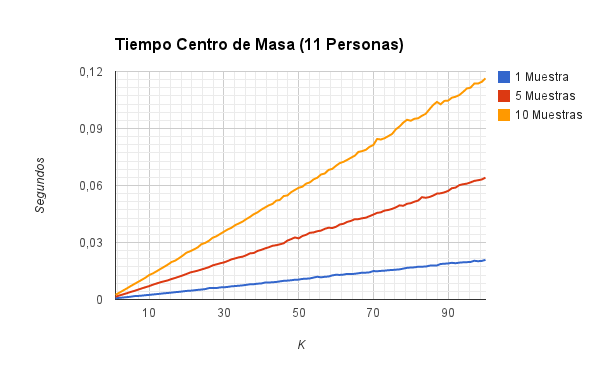
\includegraphics[width=1\textwidth]{img/image7.png} \caption{Tiempos Centro con
    Matrix $A^tA$ con 11 personas variando K} \end{figure}

\begin{figure}[H] 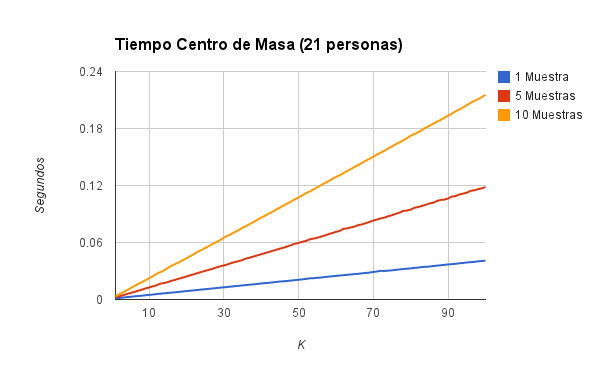
\includegraphics[width=1\textwidth]{img/image8.png} \caption{Tiempos Centro con
    Matrix $A^tA$ con 21 personas variando K} \end{figure}

\begin{figure}[H] 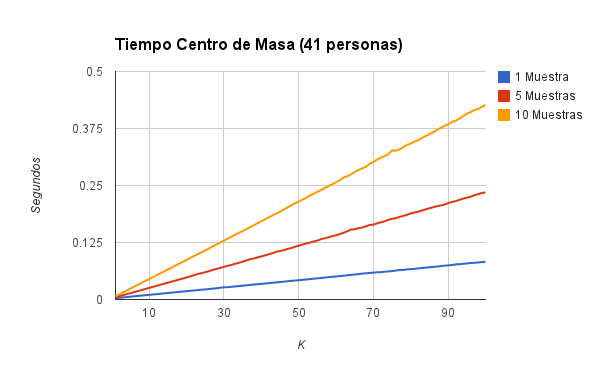
\includegraphics[width=1\textwidth]{img/image9.png} \caption{Tiempos Centro con
    Matrix $A^tA$ con 41 personas variando K} \end{figure}



Aquí pasa algo muy parecido con el caso de las mediciones de TTodos (vecino más cercano). Los
tiempos crecen a medida se incremente la cantidad de muestras, y tenemos picos, probablemente causados por un context-switch, en los
casos con pocas personas.

Si se comparan uno a uno contra los tiempos obtenidos, se ve que utilizando la distancia al centro de masa, se pueden obtener resultados en menor tiempo.

\newpage

\textbf{Mediciones de HitsTodos }

\begin{figure}[H] 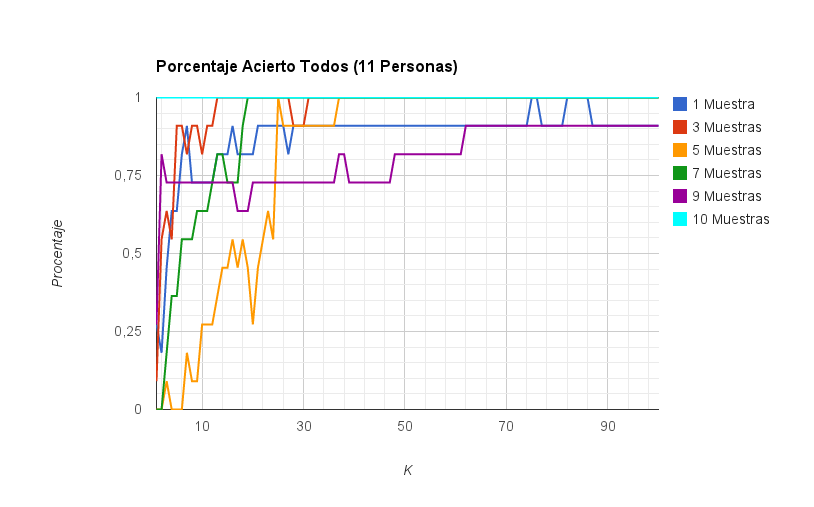
\includegraphics[width=0.90\textwidth]{img/image10.png} \caption{Coeficientes de
    efectivdad vecino más cercano con Matrix $A^tA$ con 11 personas variando K} \end{figure}

\begin{figure}[H] 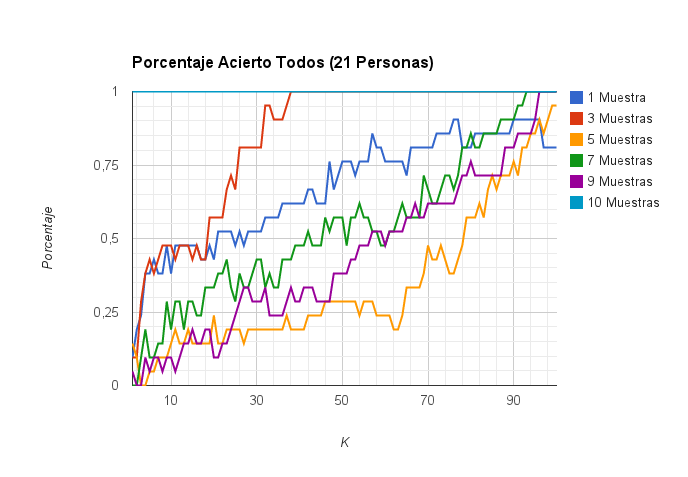
\includegraphics[width=0.90\textwidth]{img/image11.png} \caption{Coeficientes de
    efectivdad vecino más cercano con Matrix $A^tA$ con 21 personas variando K} \end{figure}

\begin{figure}[H] 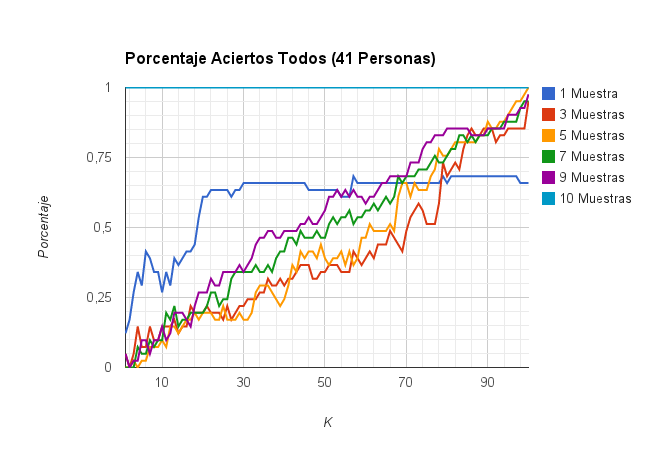
\includegraphics[width=0.90\textwidth]{img/image12.png} \caption{Coeficientes de
    efectivdad vecino más cercano con Matrix $A^tA$ con 41 personas variando K} \end{figure}

En estos tres gr\'aficos, vemos que el coeficiente de efectividad para reconocer personas, no
necesariamente mejora a medida que se incrementa k. Por ejemplo, en el gr\'afico de 11 personas, con
5 muestras hay una gran p\'erdida de efectividad entre $k=18$ y $k=20$ aproximadamente, aunque luego
mejora dr\'asticamente. Otro ejemplo ser\'ia para la misma cantidad de muestras en el caso de 21
personas, al rededor de $k=65$ y $k=75$.

Igualmente, se ve que, incrementando k, cuando hay suficientes muestras, el coeficiente de aciertos
parece tender a 1.

Por otro lado, se ve comparando los tres gr\'aficos que al aumentar la cantidad de personas a
diferenciar, se precisan m\'as autovalores para lograr el mismo coeficiente de aciertos. Esto es
esperable, dado que necesitamos m\'as informacion para diferenciar a estos.

Podemos notar tambi\'en que para las 10 muestras el coeficiente de aciertos es 1, ya que se compara
con una imagen que esta en la base de datos, esto es lo esperado en este caso ya que al ser iguales
su distancia es cero, o sea es la mas parecida.

\newpage

\textbf{Mediciones de HitsCentro }

\begin{figure}[H] 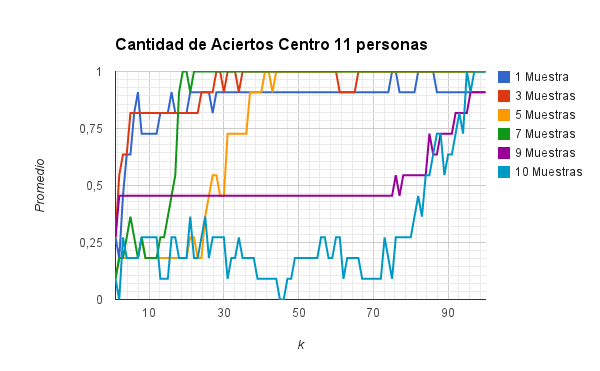
\includegraphics[width=1\textwidth]{img/image13.png} \caption{Coeficientes de
    efectivdad de Centros de Masa con Matrix $A^tA$ con 11 personas variando K} \end{figure}

\begin{figure}[H] 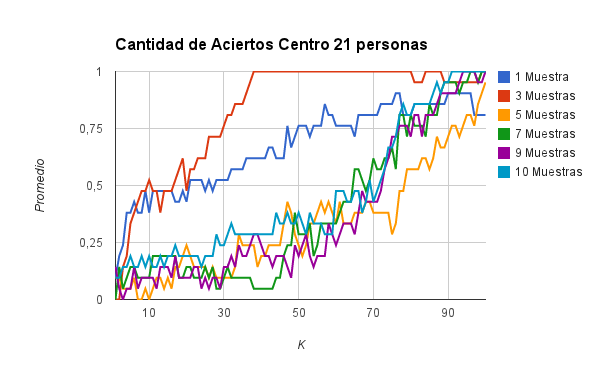
\includegraphics[width=1\textwidth]{img/image14.png} \caption{Coeficientes de
    efectivdad de Centros de Masa con Matrix $A^tA$ con 21 personas variando K} \end{figure}

\begin{figure}[H] 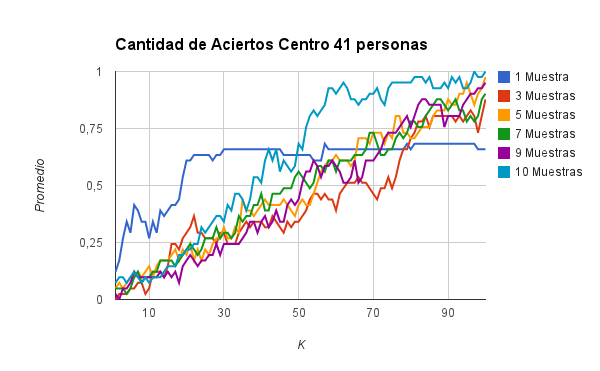
\includegraphics[width=1\textwidth]{img/image15.png} \caption{Coeficientes de
    efectivdad de Centros de Masa con Matrix $A^tA$ con 41 personas variando K} \end{figure}

El comportamiento es similar al analizado en el caso anterior, a diferencia que en los distintos
casos, la tendencia al coeficiente de aciertos 1 es m\'as lenta, o sea, precisa m\'as autovalores
para lograr los mismos resultados.

Una diferencia con el caso anterior, es que usando 10 muestras no obtenemos una efectividad del
100\% para cualquier cantidad de autovectores. Esto se debe a que si las coordenadas de una persona
a identificar, est\'an m\'as cerca del centro de masa de otra persona, este m\'etodo falla dado que
no aprecia la distruci\'on de los conjuntos pertinentes.

En el caso del m\'etodo de vecinos mas cercanos, si las distribuciones son disjuntas, en la mayor\'ia
encontraremos un vecino m\'as cerca de la persona, que del otro conjunto. Si usamos las diez muestras, la imagen ya
pertenece y por ende logramos el cien por ciento de efectividad.


\subsubsection{M\'etodo 1: Utilizando $AA^t$}

\textbf{Mediciones de TK }

\begin{figure}[H] 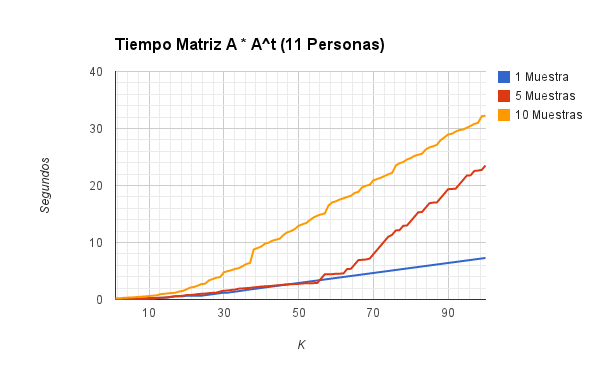
\includegraphics[width=1\textwidth]{img/imagea.png} \caption{Tiempos Matrix $AA^t$
    con 11 personas variando K} \end{figure}

\begin{figure}[H] 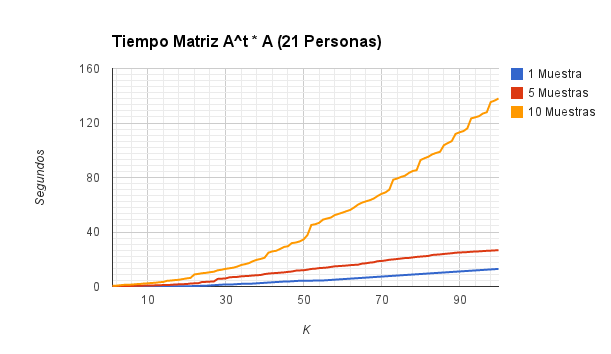
\includegraphics[width=1\textwidth]{img/imageb.png} \caption{Tiempos Matrix $AA^t$
    con 21 personas variando K} \end{figure}

\begin{figure}[H] 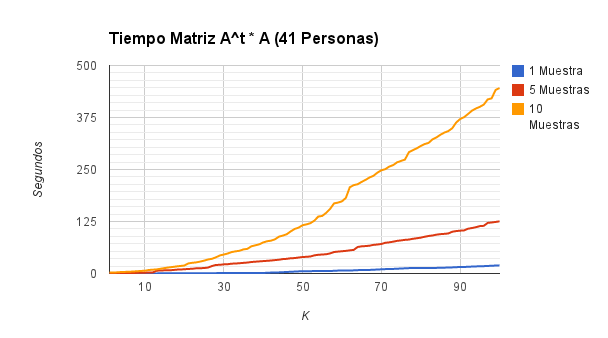
\includegraphics[width=1\textwidth]{img/imagec.png} \caption{Tiempos Matrix $AA^t$
    con 41 personas variando K} \end{figure}

A diferencia de antes, la matriz utilizada dentro del m\'etodo de la potencia, $A A^t$ en este caso,
tiene un tama\~no menor pero no constante y ahora sí depende de cu\'an robusta es la base de datos.
Esta medida es $Personas \times Muestras$.

Otra diferencia es que en estos gráficos los tests tardan más mientras mayor sea la cantidad de
muestras. Esto se debe a que aunque menor cantidad de muestras implica menor cantidad de
autovectores y finalmente implicaría mayor cantidad de iteraciones para el método de la potencia, la
matriz termina siendo mucho más chica; tanto que la diferencia entre hacer 10.000 iteraciones para
una matriz chica y 200 iteraciones para una matriz grande es mucho mayor.


\textbf{Mediciones de Ttodos }

\begin{figure}[H] 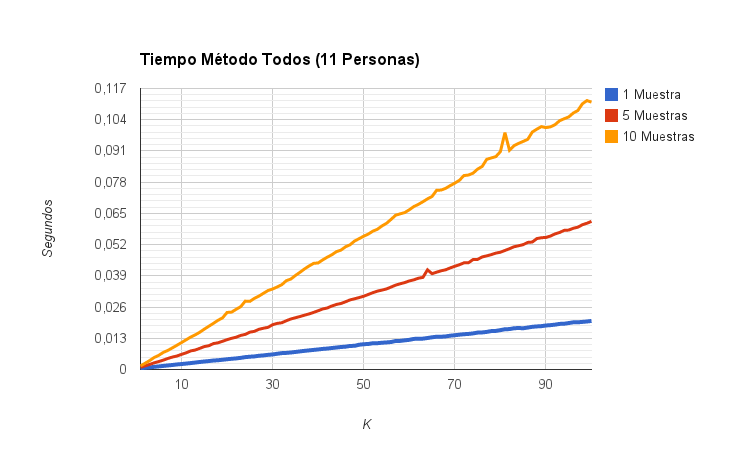
\includegraphics[width=1\textwidth]{img/imaged.png} \caption{Tiempos Todos con
    Matrix $AA^t$ con 11 personas variando K} \end{figure}

\begin{figure}[H] 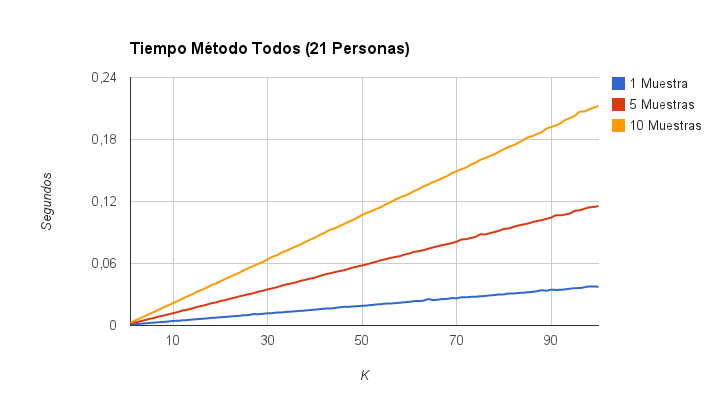
\includegraphics[width=1\textwidth]{img/imagee.png} \caption{Tiempos Todos con
    Matrix $AA^t$ con 21 personas variando K} \end{figure}

\begin{figure}[H] 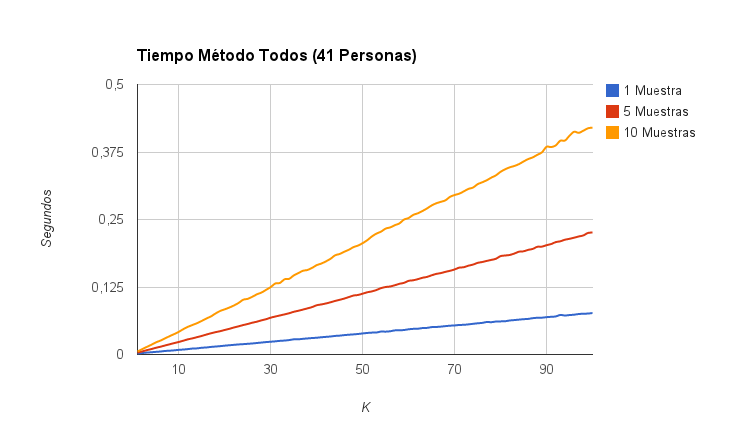
\includegraphics[width=1\textwidth]{img/imagef.png} \caption{Tiempos Todos con
    Matrix $AA^t$ con 41 personas variando K} \end{figure}

No se notan muchos cambios con el método 0. Esto se debe a que los autovectores terminarían casi identicos, sin importar el método 0 o método 1. En consecuencia, los tiempos son muy similares, dado que las operaciones
aplicadas sobre ellos son exactamente las mismas.

\textbf{Mediciones de Tcentro }

\begin{figure}[H] 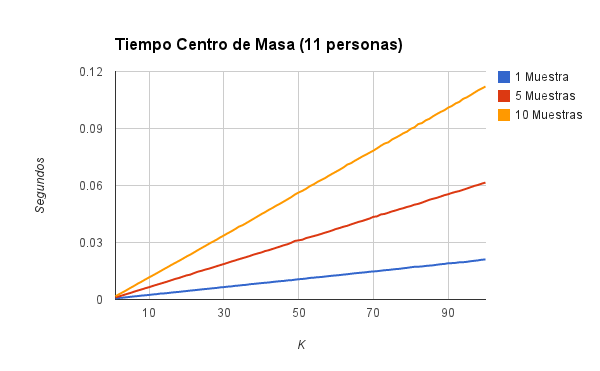
\includegraphics[width=1\textwidth]{img/imageg.png} \caption{Tiempos Centro con
    Matrix $AA^t$ con 11 personas variando K} \end{figure}

\begin{figure}[H] 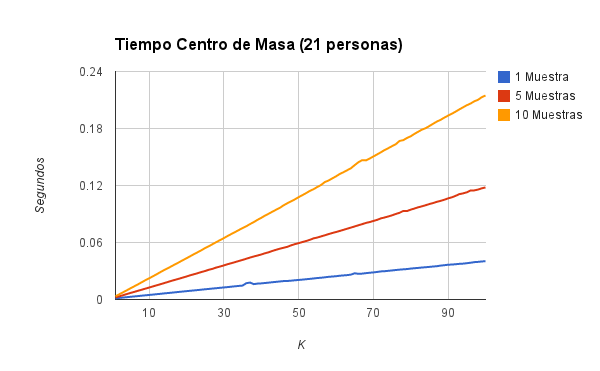
\includegraphics[width=1\textwidth]{img/imageh.png} \caption{Tiempos Centro con
    Matrix $AA^t$ con 21 personas variando K} \end{figure}

\begin{figure}[H] 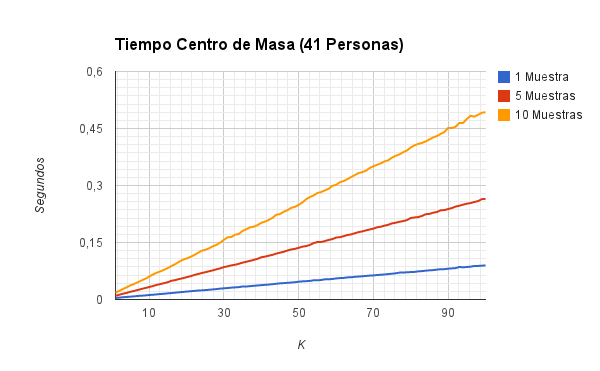
\includegraphics[width=1\textwidth]{img/imagei.png} \caption{Tiempos Centro con
    Matrix $AA^t$ con 41 personas variando K} \end{figure}

Ocurre lo mismo que con el tiempo de Ttodos (vecino más cercano).

\textbf{Mediciones de HitsTodos}

\begin{figure}[H] 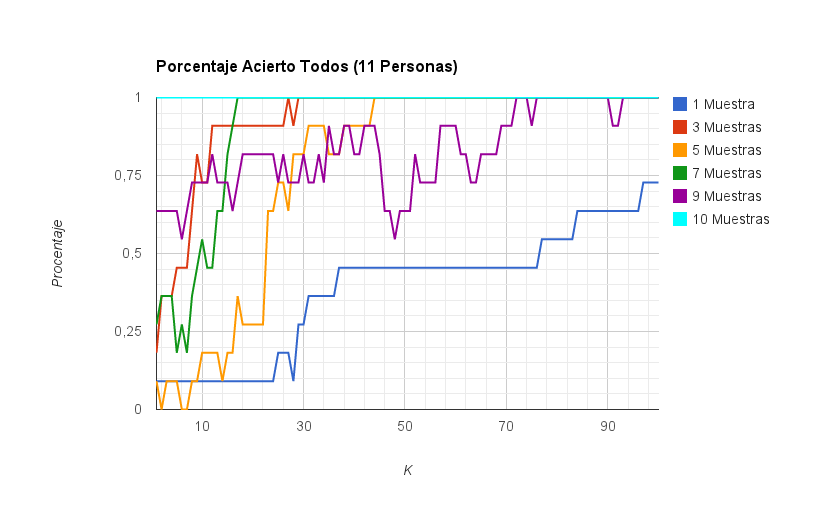
\includegraphics[width=0.9\textwidth]{img/imagej.png} \caption{Coeficientes de
    efectivdad vecino más cercano con Matrix $AA^t$ con 11 personas variando K} \end{figure}

\begin{figure}[H] 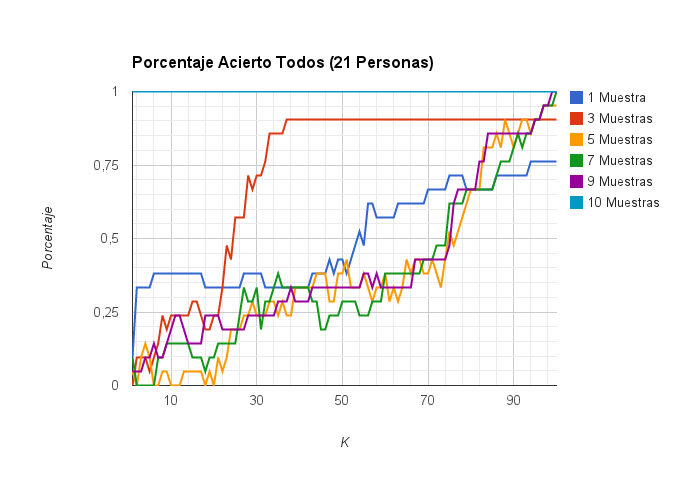
\includegraphics[width=0.9\textwidth]{img/imagek.png} \caption{Coeficientes de
    efectivdad vecino más cercano con Matrix $AA^t$ con 21 personas variando K} \end{figure}

\begin{figure}[H] 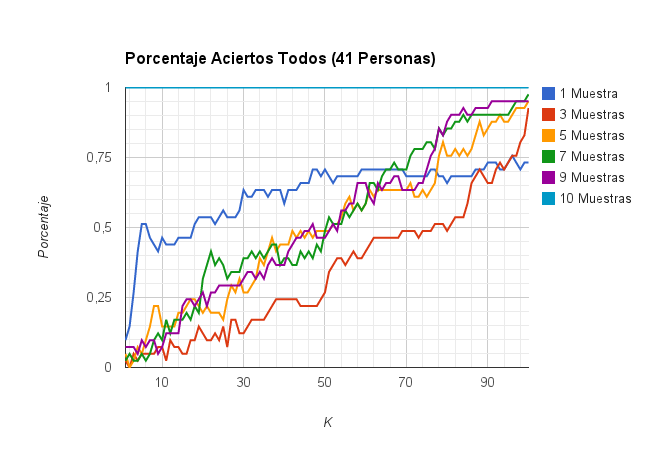
\includegraphics[width=0.9\textwidth]{img/imagel.png} \caption{Coeficientes de
    efectivdad vecino más cercano con Matrix $AA^t$ con 41 personas variando K} \end{figure}

Notamos que el comportamiento es muy parecido al comportamientos del M\'etodo 0, entre otras cosas
vemos que al incrementar el k el coeficiente de aciertos tiene a 1.  Un detalle que notamos que
tiene diferencia con el M\'etodo 0, es que para algunos valores de muestra chicos, como por ejemplo
Grafico 1 con 1 muestra o Grafico 2 con 3 muestras, le cuesta mas aumentar el porcentaje de
aciertos.

Podemos notar  que para las 10 muestras el porcentaje de aciertos es el 100 porciento ya que se
compara con una imagen que esta en la base de datos.

\newpage

\textbf{Mediciones de HitsCentro}

\begin{figure}[H] 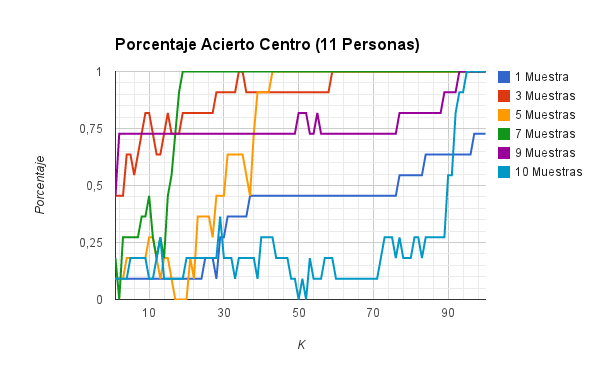
\includegraphics[width=1\textwidth]{img/imagem.png} \caption{Coeficientes de
    efectivdad de Centros de Masa con Matrix $AA^t$ con 11 personas variando K} \end{figure}

\begin{figure}[H] 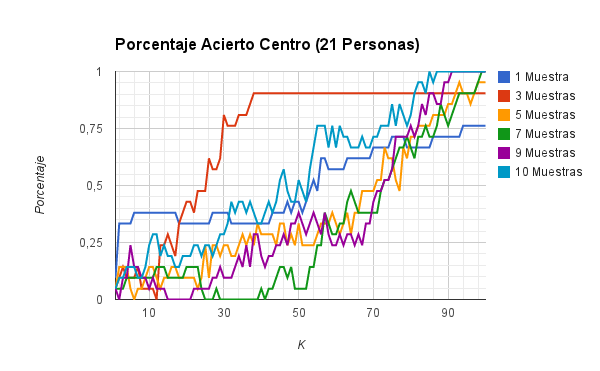
\includegraphics[width=1\textwidth]{img/imagen.png} \caption{Coeficientes de
    efectivdad de Centros de Masa Matrix $AA^t$ con 21 personas variando K} \end{figure}

\begin{figure}[H] 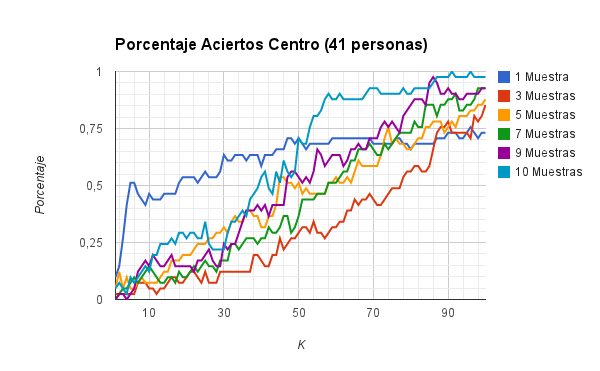
\includegraphics[width=1\textwidth]{img/imager.png} \caption{Coeficientes de
    efectividad de Centros de Masa con Matrix $AA^t$ con 41 personas variando K} \end{figure}

Al igual que los graficos anteriores, estos graficos se comportan muy similar a los del M\'etodo 0,
quiza en algunos casos particulares (como por ejemplo, Grafico 1 con 9 muestras) se tiene un
porcentaje de acierto mas alto y en otros casos (como por ejemplo, Grafico 1 con 1 muestra) se tiene
un porcentaje de acierto mas bajo. Pero en general los porcentajes entre este m\'etodo y el anterior
son similares.



%%%%%%%%% ------------------------------------- %%%%%%%%%%%%%%%%%%%%%%%%%%%%%
\subsection{Experimentacion con Imagenes Full}

\subsubsection{M\'etodo 0: Utilizando $A^tA$}

Estos tests no los realizamos ya que el tiempo de ejecucion es muy elevado y ademas vamos  a obtener
los mismos resultados que a los aplicados con el \textbf{m\'etodo 1} por lo demostrado en el lema: \\
\\ \textbf{Lema:} Si $u$ es autovector de $A A^t$ con $\lambda$ autovalor asociado, entonces $A^t u
\in \mathbb{R}^m$ es autovector de $A^t A$ también con $\lambda$ autovalor asociado.  \\ \\ el cual
esta demostrado en la seccion \textbf{Demostraciones}
 
Notamos que el comportamiento es el mismo que en las imagenes reducidas.

%%%%%%%%%%%%%%%%% *********** %%%%%%%%%%%%%%%%%
\subsubsection{M\'etodo 1: Utilizando $AA^t$}

\textbf{Mediciones de TK}

\begin{figure}[H] 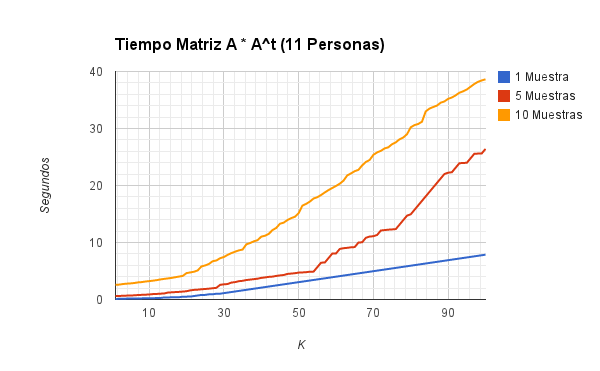
\includegraphics[width=1\textwidth]{img/imagef1.png} \caption{Tiempos de calcular
    la Matrix $AA^t$ con 11 personas variando K} \end{figure}

\begin{figure}[H] 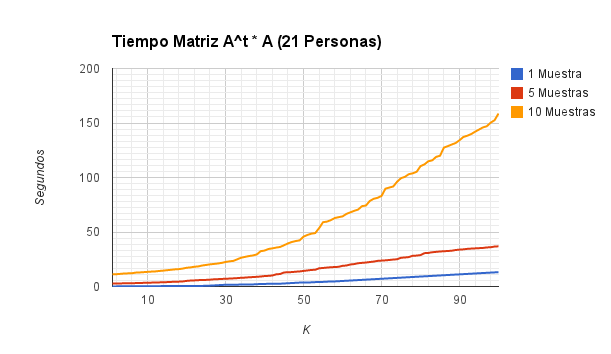
\includegraphics[width=1\textwidth]{img/imagef2.png} \caption{Tiempos de calcular
    la Matrix $AA^t$ con 21 personas variando K} \end{figure}

\begin{figure}[H] 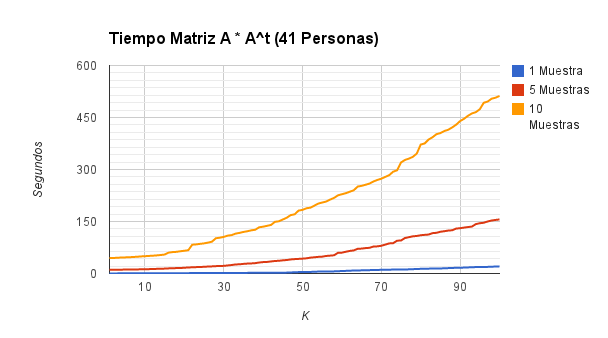
\includegraphics[width=1\textwidth]{img/imagef3.png} \caption{Tiempos de calcular
    la Matrix $AA^t$ con 41 personas variando K} \end{figure}

Si comparamos estas 3 imágenes con las hechas por el método 1 sobre las imágenes de menor resolución
veremos que describen el mismo comportamiento. Lo que vale
la pena notar es que la diferencia de tiemops no es muy grande, en el gráfico para 11 personas, el
máximo tiempo es de 33 segundos aproximadamente para el de resoluciones pequeñas y 40 para el caso
de las resoluciones grandes, con un crecimiento similar. Algo parecido sucede con 21 y 41 personas.
Esto es un hecho digno de remarcar dado que las imágenes tienen mil veces menos pixeles en el primer
caso. El causante de que el incremento sea tan peque\~no es que s\'olo se opera con la matriz de gran resoluci\'on al realizar las operaciones necesarias del producto $AA^t$, luego se operan en ambos casos matrices de igual tama\~no.

\textbf{Mediciones de Ttodos }

\begin{figure}[H] 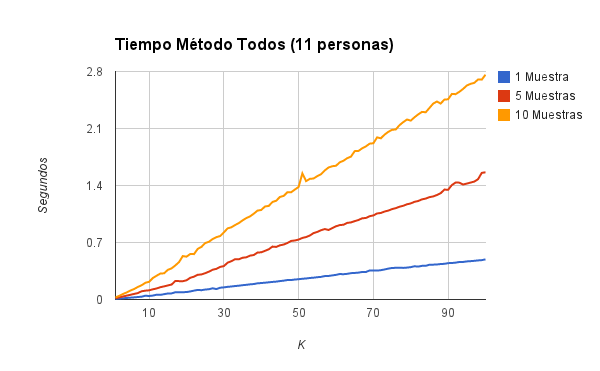
\includegraphics[width=1\textwidth]{img/imagef4.png} \caption{Tiempos de vecino
    más cercano con Matrix $AA^t$ con 11 personas variando K} \end{figure}

\begin{figure}[H] 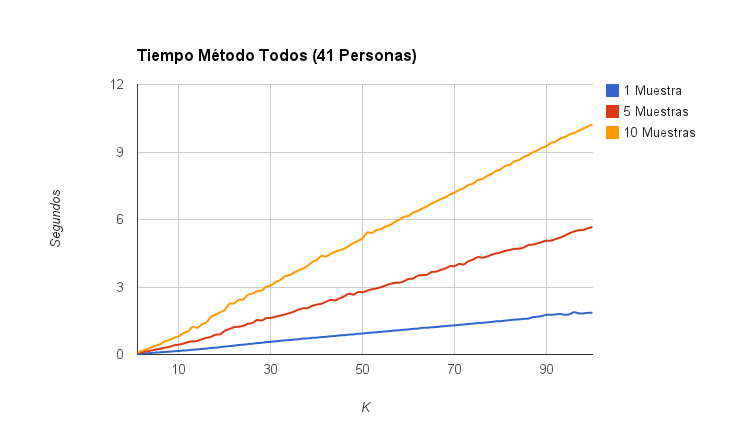
\includegraphics[width=1\textwidth]{img/imagef5.png} \caption{Tiempos de vecino
    más cercano Matrix $AA^t$ con 21 personas variando K} \end{figure}

\begin{figure}[H] 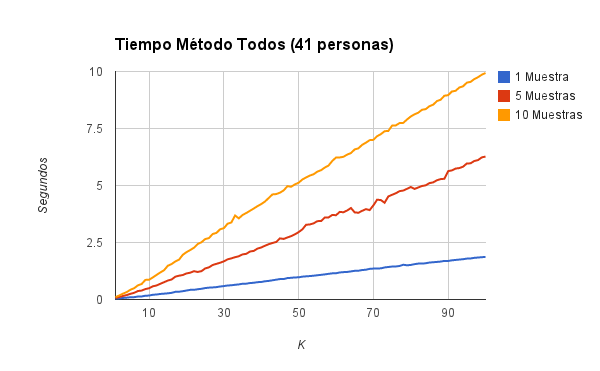
\includegraphics[width=1\textwidth]{img/imagef6.png} \caption{Tiempos de vecino
    más cercano Matrix $AA^t$ con 41 personas variando K} \end{figure}

De nuevo aparentarían ser gráficos muy parecidos, sólo que en este caso la constante de crecimiento es mayor.
Por ejemplo, con 11 personas, 2,88 segundos es el máximo en el caso de mayores resoluciones mientras
que era  0.117 en el de menores resoluciones.  Esto tiene sentido dado que las dimensiones de cada
imagen es mayor, lo que implica mayor tiempo para restarle $\mu$ y dividirlo por $\sqrt{n-1}$, y
también mayor tiempo para hacer el cambio de bases de ellos.

\textbf{Mediciones de Tcentro }

\begin{figure}[H] 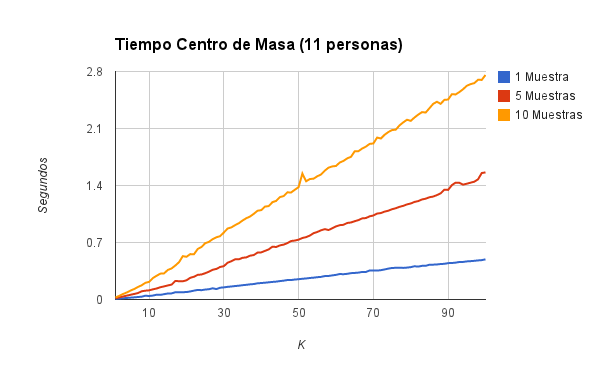
\includegraphics[width=1\textwidth]{img/imagef7.png} \caption{Tiempos de Centros
    de Masa Matrix $AA^t$ con 11 personas variando K} \end{figure}

\begin{figure}[H] 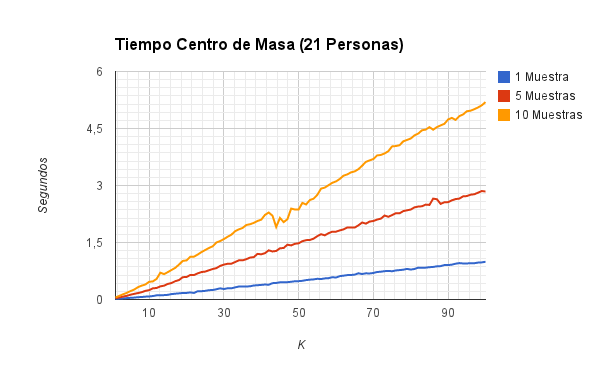
\includegraphics[width=1\textwidth]{img/imagef8.png} \caption{Tiempos de Centros
    de Masa con Matrix $AA^t$ con 21 personas variando K} \end{figure}

\begin{figure}[H] 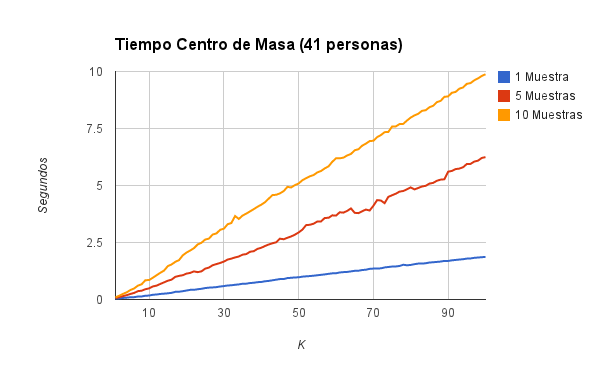
\includegraphics[width=1\textwidth]{img/imagef9.png} \caption{Tiempos de Centros
    de Masa con Matrix $AA^t$ con 41 personas variando K} \end{figure}

De nuevo, muy similares a los tests con baja resolución sólo que con constante de costo algor\'itmico notablemente mayor.

\textbf{Mediciones de HitsTodos. }

\begin{figure}[H] 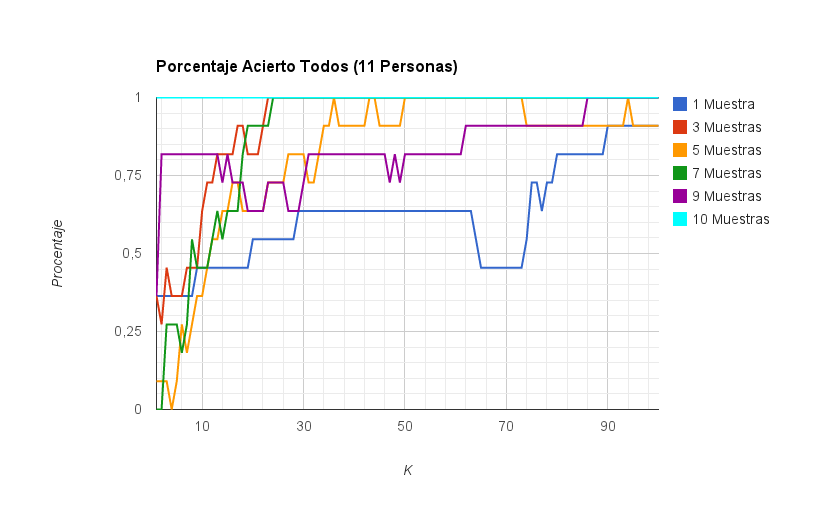
\includegraphics[width=0.9\textwidth]{img/imagef10.png} \caption{Coeficiente de
    efectividad de Vecino Más Cercano con Matrix $AA^t$ con 11 personas variando K} \end{figure}

\begin{figure}[H] 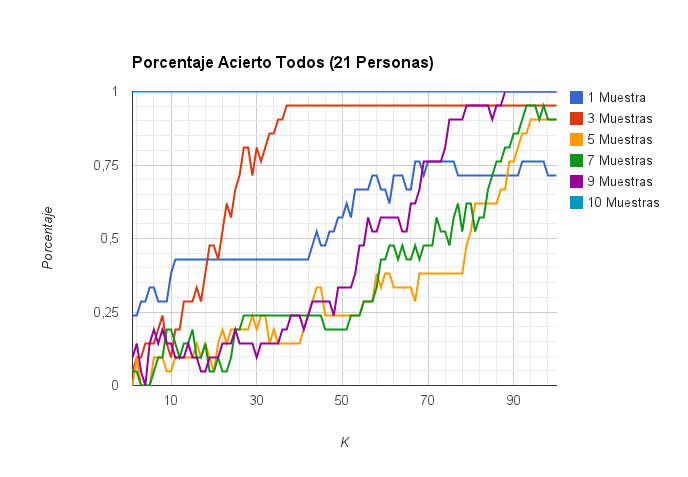
\includegraphics[width=0.9\textwidth]{img/imagef11.png} \caption{Coeficiente de
    efectividad de Vecino Más Cercano Matrix $AA^t$ con 21 personas variando K} \end{figure}

\begin{figure}[H] 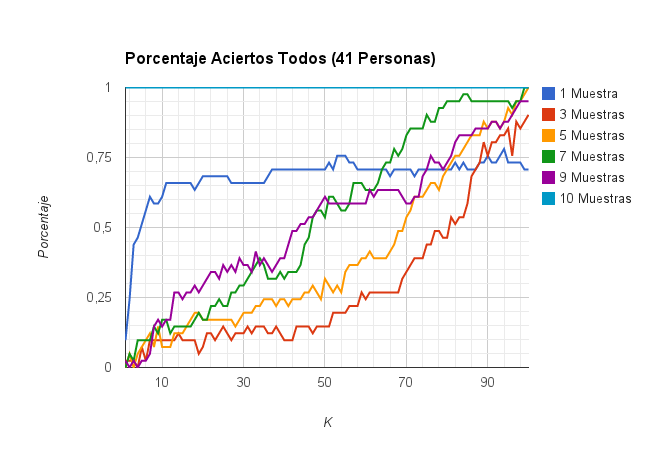
\includegraphics[width=0.9\textwidth]{img/imagef12.png} \caption{Coeficiente de
    efectividad de Vecino Más Cercano con Matrix $AA^t$ con 41 personas variando K} \end{figure}

Comparándolos con los gráficos de menor resolución con método 1 como veníamos haciendo, son a simple vista muy similares. En el gráfico con 11 personas, el test con una muestra se toma su tiempo para ir
incrementando su efectividad acorde sube el K mientras que los otros suben mucho más empinadamente.

En el gráfico de 21 personas, de nuevo es muy parecido. El caso con 3 muestras sube rápidamente y
luego se estanca en una efectividad menor a 1, mientras que el resto sube lentamente hasta llegar a
una efectividad de 1, con excepción del test con una muestra en ambos casos.

En el caso de 41 personas tampoco hay mucho para decir. Muy parecido a los tests 
con resoluciones pequeñas.

Esta similitud contradice un poco la noción de que mayor resolución de las imágenes implica una
mayor efectividad al identificar sujetos. Sin embargo, aquí no se ve esa diferencia en eficacia. Las
posibles razones podrían ser que los primeros autovectores de ambas versiones de las imágenes
acumulan la misma cantidad de varianza, y por ende, la misma cantidad de autovectores nos resumiría
la misma información en ambos casos. Se debería hacer tests más específicos para poder confirmar
ésta u otra hipótesis.

\newpage

\textbf{Mediciones de HitsCentro }

\begin{figure}[H] 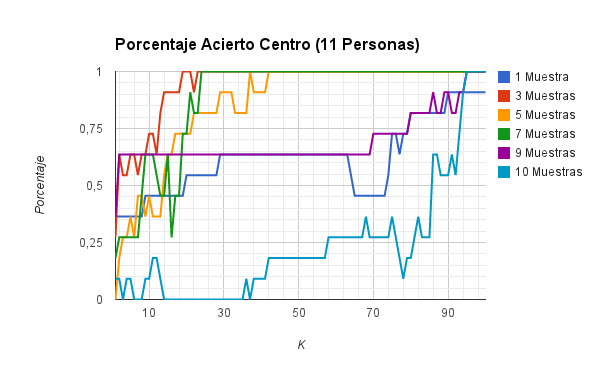
\includegraphics[width=1\textwidth]{img/imagef13.png} \caption{Coeficiente de
    efectividad de Centros de Masa con Matrix $AA^t$ con 11 personas variando K} \end{figure}

\begin{figure}[H] 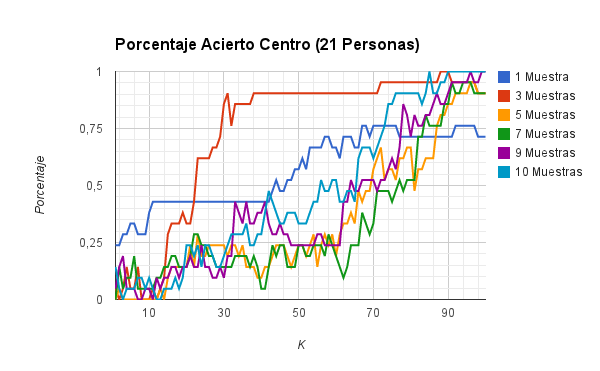
\includegraphics[width=1\textwidth]{img/imagef14.png} \caption{Coeficiente de
    efectividad de Centros de Masa con Matrix $AA^t$ con 21 personas variando K} \end{figure}

\begin{figure}[H] 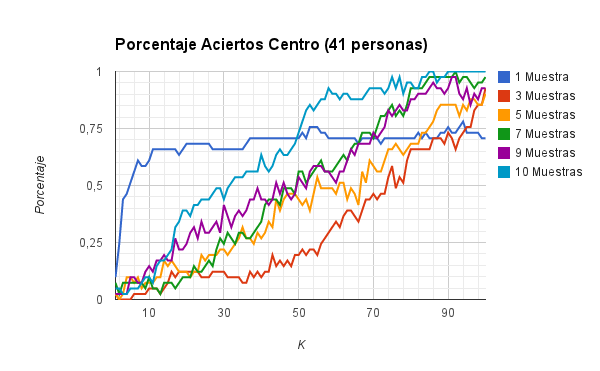
\includegraphics[width=1\textwidth]{img/imagef15.png} \caption{Coeficiente de
    efectividad de Centros de Masa  con Matrix $AA^t$ con 41 personas variando K} \end{figure}


Ya en nuestros últimos tests notamos la misma tendencia. La pinta uno a uno con 11, 21 y 41 personas
es de nuevo muy similar. Las razones de esto podrían ser las mismas que en el caso de la efectividad
del vecino más cercano.


\subsection{Conclusiones}

En conclusión, el método 0 y el método 1 son intercambiables para el reconocimiento de rostros, pero
el primero conlleva una necesidad de cómputo mucho mayor al segundo. Esto inclinaría la balanza
claramente en favor del método 1 y no se verían razones por las cuales usar el método 0, dado que se introduce un peque\~o error al cambiar de espacios, no son tan da\~ninos como para no poder ser superados utilizando m\'as autovalores.

Sobre el reconocimiento de rostros en sí, no se consiguió una efectividad tan alta como se
esperaba con una peque\~na cantidad de autovectores, se necesitan 90 o más para lograr una efectividad de al menos el 75\% sin importar
la cantidad de muestras. Sin embargo, la cantidad de muestras sí parece influir en qué tan bueno es
el reconocimiento, aunque conlleva un costo de cómputo mayor. Quedaría en el usuario de estos
métodos decidir si el costo de tiempo es un precio que están dispuestos a pagar o no, dependiendo de
las exigencias del uso elegido.

Respecto a los m\'etodos de reconocimiento, utilizar el centro de masas s\'olo dar\'a \'optimos resultados si se logra con gr\'an cantidad de autovalores, alejar las muestras es decir, cuando cambiamos de espacio todos los puntos que corresponden a una misma persona est\'en bien alejados alejados de los puntos de otras personas, en otras palabras una distribuci\'on que representa a una persona es disjunta de las dem\'as, dado el tiempo requerido en construir la base de datos, quizas no es tan costoso optar por un m\'etodo m\'as lento que precise menos autovalores para conseguir los mismos resultados, como el de comparar contra todas las muestras, o uno m\'as sofisticado. Por cierto, aqu\'i podr\'ian ya utilizarse m\'etodos para paralelizar estas cuentas(b\'usqueda de la m\i'nima distancia) que no son as\' aplicables aparentemente en el m\'etodo de la potencia, salvo en las propias operaciones matriciales.

Otro experimento interesante a realizar, ser\'ia exponer un m\'etodo de reconocimiento que pueda diferenciar, dadas las distribuciones conocidas, si una nueva muestra no pertenece a los sujetos que se encuentran ya en la base de datos.

